% Created 2024-10-16 śro 21:35
% Intended LaTeX compiler: pdflatex
\documentclass[../../main.tex]{subfiles}

% \usepackage[a4paper, margin=3cm]{geometry}
% \usepackage{amssymb} // not working

\usepackage[T1]{fontenc}
\usepackage[utf8]{inputenc}
\usepackage{graphicx}
\usepackage{longtable}
\usepackage{wrapfig}
\usepackage{rotating}
\usepackage[normalem]{ulem}
\usepackage{amsmath}
\usepackage{capt-of}
\usepackage{hyperref}
\usepackage{siunitx}
\usepackage{float}
\usepackage[polish]{babel}

\graphicspath{{../}}
\author{Wojciech Paderewski}
\date{\today}
\title{Koncepcja ukladu}
\hypersetup{
 pdfauthor={Wojciech Paderewski},
 pdftitle={Koncepcja ukladu},
 pdfkeywords={},
 pdfsubject={},
 pdflang={Polish}}

\begin{document}

\subsection{Złącze USB-C do programowania}
\subsubsection{Dobór złącza}
Złącze usb musi posiadac przynajmniej 12 pinów, ponieważ dopiero w takim układzie jest na złączu są linie D+ i D-, czyli linie danych.
Wybrano złącze 16 pinowe, ponieważ takie było dostępne w sklepie.
\subsubsection{Opis podłączenia}
Złącze USB-C będzie podłączone bezpośrednio do ESP32-S3, ponieważ posiada on wbudowany programator.
By ustawić napięcie komunikacji USB-C na 3.3V, zastosowano rezystory podciągające R1 i R2 o wartości 5.1k$\Omega$.
Do podłączenia wykorzystano parę różnicową by połączyć linie D+ i D- z ESP32-S3, w celu zminimalizowania zakłóceń CMN (Common Mode Noise).
\subsubsection{Zabezpieczenia ESD}
W celu zabezpieczenia linii przed przepięciami, zastosowano diody TVS PUSB3AB4Z firmy Nexperia. Diody te mają wystarczająco duże opakowanie by dało się je zlutować ręcznie, napięciem roboczym jest 3.3V,
a napięcie stabilizacji wynosi 5V.

Mimo że jest to napięcie wyższe niż napięcie zasilania ESP32-S3, to nie powinno to stanowić problemu, 
ponieważ napięcie to pojawi się na krótki czas, a sam esp32-s3 ma również wbudowane zabezpieczenia przed przepięciami.

Wewnętrzne zabezpieczenia według noty katalogowej ESP32-S3:
\begin{itemize}
    \item Test Standard JS-001; HBM (Human Body Mode) ± 2000 V
    \item Test Standard JS-002; CDM (Charged Device Model) ± 1000 V
\end{itemize}
Wynika z tego, że złącze USB-C w dość dobry sposób jest zabezpieczone przed przepięciami.
\subsubsection{Schemat}
\begin{figure}[H]
    \centering
    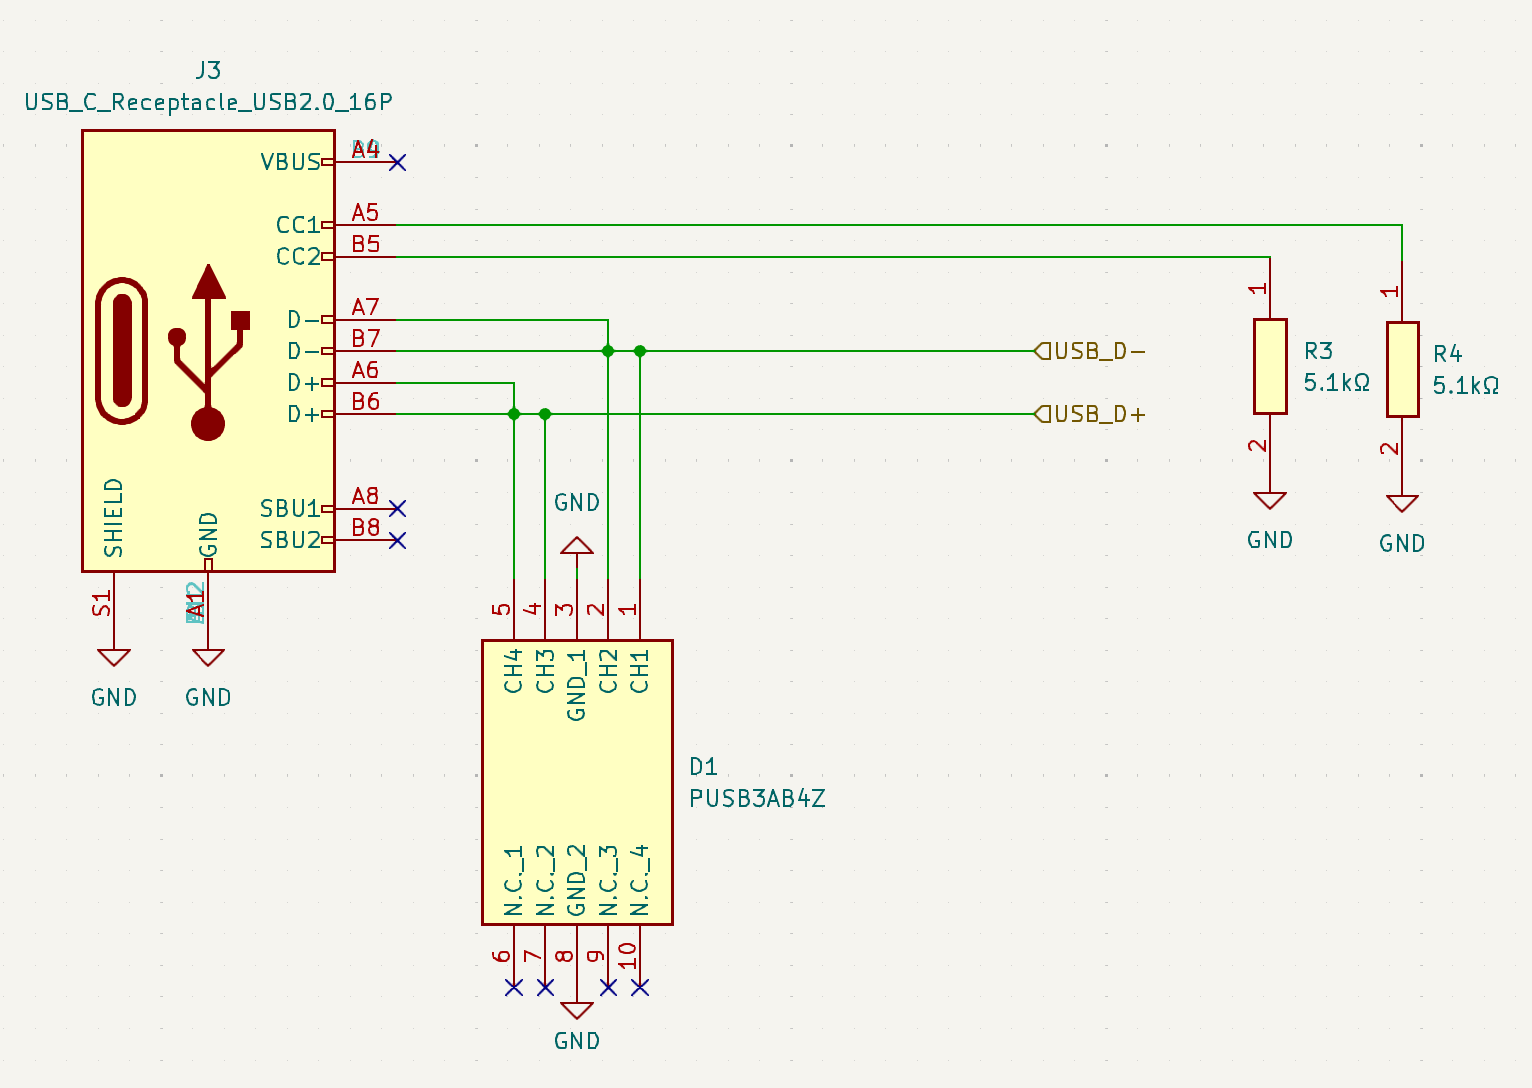
\includegraphics[width=0.8\textwidth]{usb-c_schemat.png}
    \caption{Schemat złącza USB-C do programowania}
\end{figure}
\end{document}
